
%% bare_conf.tex
%% V1.4b
%% 2015/08/26
%% by Michael Shell
%% See:
%% http://www.michaelshell.org/
%% for current contact information.
%%
%% This is a skeleton file demonstrating the use of IEEEtran.cls
%% (requires IEEEtran.cls version 1.8b or later) with an IEEE
%% conference paper.
%%
%% Support sites:
%% http://www.michaelshell.org/tex/ieeetran/
%% http://www.ctan.org/pkg/ieeetran
%% and
%% http://www.ieee.org/

%%*************************************************************************
%% Legal Notice:
%% This code is offered as-is without any warranty either expressed or
%% implied; without even the implied warranty of MERCHANTABILITY or
%% FITNESS FOR A PARTICULAR PURPOSE! 
%% User assumes all risk.
%% In no event shall the IEEE or any contributor to this code be liable for
%% any damages or losses, including, but not limited to, incidental,
%% consequential, or any other damages, resulting from the use or misuse
%% of any information contained here.
%%
%% All comments are the opinions of their respective authors and are not
%% necessarily endorsed by the IEEE.
%%
%% This work is distributed under the LaTeX Project Public License (LPPL)
%% ( http://www.latex-project.org/ ) version 1.3, and may be freely used,
%% distributed and modified. A copy of the LPPL, version 1.3, is included
%% in the base LaTeX documentation of all distributions of LaTeX released
%% 2003/12/01 or later.
%% Retain all contribution notices and credits.
%% ** Modified files should be clearly indicated as such, including  **
%% ** renaming them and changing author support contact information. **
%%*************************************************************************


% *** Authors should verify (and, if needed, correct) their LaTeX system  ***
% *** with the testflow diagnostic prior to trusting their LaTeX platform ***
% *** with production work. The IEEE's font choices and paper sizes can   ***
% *** trigger bugs that do not appear when using other class files.       ***                          ***
% The testflow support page is at:
% http://www.michaelshell.org/tex/testflow/



\documentclass[conference]{IEEEtran}
\usepackage[utf8]{inputenc}
\usepackage[T1]{fontenc}
% Some Computer Society conferences also require the compsoc mode option,
% but others use the standard conference format.
%
% If IEEEtran.cls has not been installed into the LaTeX system files,
% manually specify the path to it like:
% \documentclass[conference]{../sty/IEEEtran}





% Some very useful LaTeX packages include:
% (uncomment the ones you want to load)


% *** MISC UTILITY PACKAGES ***
%
%\usepackage{ifpdf}
% Heiko Oberdiek's ifpdf.sty is very useful if you need conditional
% compilation based on whether the output is pdf or dvi.
% usage:
% \ifpdf
%   % pdf code
% \else
%   % dvi code
% \fi
% The latest version of ifpdf.sty can be obtained from:
% http://www.ctan.org/pkg/ifpdf
% Also, note that IEEEtran.cls V1.7 and later provides a builtin
% \ifCLASSINFOpdf conditional that works the same way.
% When switching from latex to pdflatex and vice-versa, the compiler may
% have to be run twice to clear warning/error messages.






% *** CITATION PACKAGES ***

\usepackage{cite}
% cite.sty was written by Donald Arseneau
% V1.6 and later of IEEEtran pre-defines the format of the cite.sty package
% \cite{} output to follow that of the IEEE. Loading the cite package will
% result in citation numbers being automatically sorted and properly
% "compressed/ranged". e.g., [1], [9], [2], [7], [5], [6] without using
% cite.sty will become [1], [2], [5]--[7], [9] using cite.sty. cite.sty's
% \cite will automatically add leading space, if needed. Use cite.sty's
% noadjust option (cite.sty V3.8 and later) if you want to turn this off
% such as if a citation ever needs to be enclosed in parenthesis.
% cite.sty is already installed on most LaTeX systems. Be sure and use
% version 5.0 (2009-03-20) and later if using hyperref.sty.
% The latest version can be obtained at:
% http://www.ctan.org/pkg/cite
% The documentation is contained in the cite.sty file itself.






% *** GRAPHICS RELATED PACKAGES ***
%
\ifCLASSINFOpdf
  % \usepackage[pdftex]{graphicx}
  % declare the path(s) where your graphic files are
  % \graphicspath{{../pdf/}{../jpeg/}}
  % and their extensions so you won't have to specify these with
  % every instance of \includegraphics
  % \DeclareGraphicsExtensions{.pdf,.jpeg,.png}
\else
  % or other class option (dvipsone, dvipdf, if not using dvips). graphicx
  % will default to the driver specified in the system graphics.cfg if no
  % driver is specified.
  % \usepackage[dvips]{graphicx}
  % declare the path(s) where your graphic files are
  % \graphicspath{{../eps/}}
  % and their extensions so you won't have to specify these with
  % every instance of \includegraphics
  % \DeclareGraphicsExtensions{.eps}
\fi
% graphicx was written by David Carlisle and Sebastian Rahtz. It is
% required if you want graphics, photos, etc. graphicx.sty is already
% installed on most LaTeX systems. The latest version and documentation
% can be obtained at: 
% http://www.ctan.org/pkg/graphicx
% Another good source of documentation is "Using Imported Graphics in
% LaTeX2e" by Keith Reckdahl which can be found at:
% http://www.ctan.org/pkg/epslatex
%
% latex, and pdflatex in dvi mode, support graphics in encapsulated
% postscript (.eps) format. pdflatex in pdf mode supports graphics
% in .pdf, .jpeg, .png and .mps (metapost) formats. Users should ensure
% that all non-photo figures use a vector format (.eps, .pdf, .mps) and
% not a bitmapped formats (.jpeg, .png). The IEEE frowns on bitmapped formats
% which can result in "jaggedy"/blurry rendering of lines and letters as
% well as large increases in file sizes.
%
% You can find documentation about the pdfTeX application at:
% http://www.tug.org/applications/pdftex





% *** MATH PACKAGES ***
%
%\usepackage{amsmath}
% A popular package from the American Mathematical Society that provides
% many useful and powerful commands for dealing with mathematics.
%
% Note that the amsmath package sets \interdisplaylinepenalty to 10000
% thus preventing page breaks from occurring within multiline equations. Use:
%\interdisplaylinepenalty=2500
% after loading amsmath to restore such page breaks as IEEEtran.cls normally
% does. amsmath.sty is already installed on most LaTeX systems. The latest
% version and documentation can be obtained at:
% http://www.ctan.org/pkg/amsmath





% *** SPECIALIZED LIST PACKAGES ***
%
%\usepackage{algorithmic}
% algorithmic.sty was written by Peter Williams and Rogerio Brito.
% This package provides an algorithmic environment fo describing algorithms.
% You can use the algorithmic environment in-text or within a figure
% environment to provide for a floating algorithm. Do NOT use the algorithm
% floating environment provided by algorithm.sty (by the same authors) or
% algorithm2e.sty (by Christophe Fiorio) as the IEEE does not use dedicated
% algorithm float types and packages that provide these will not provide
% correct IEEE style captions. The latest version and documentation of
% algorithmic.sty can be obtained at:
% http://www.ctan.org/pkg/algorithms
% Also of interest may be the (relatively newer and more customizable)
% algorithmicx.sty package by Szasz Janos:
% http://www.ctan.org/pkg/algorithmicx




% *** ALIGNMENT PACKAGES ***
%
%\usepackage{array}
% Frank Mittelbach's and David Carlisle's array.sty patches and improves
% the standard LaTeX2e array and tabular environments to provide better
% appearance and additional user controls. As the default LaTeX2e table
% generation code is lacking to the point of almost being broken with
% respect to the quality of the end results, all users are strongly
% advised to use an enhanced (at the very least that provided by array.sty)
% set of table tools. array.sty is already installed on most systems. The
% latest version and documentation can be obtained at:
% http://www.ctan.org/pkg/array


% IEEEtran contains the IEEEeqnarray family of commands that can be used to
% generate multiline equations as well as matrices, tables, etc., of high
% quality.




% *** SUBFIGURE PACKAGES ***
%\ifCLASSOPTIONcompsoc
%  \usepackage[caption=false,font=normalsize,labelfont=sf,textfont=sf]{subfig}
%\else
%  \usepackage[caption=false,font=footnotesize]{subfig}
%\fi
% subfig.sty, written by Steven Douglas Cochran, is the modern replacement
% for subfigure.sty, the latter of which is no longer maintained and is
% incompatible with some LaTeX packages including fixltx2e. However,
% subfig.sty requires and automatically loads Axel Sommerfeldt's caption.sty
% which will override IEEEtran.cls' handling of captions and this will result
% in non-IEEE style figure/table captions. To prevent this problem, be sure
% and invoke subfig.sty's "caption=false" package option (available since
% subfig.sty version 1.3, 2005/06/28) as this is will preserve IEEEtran.cls
% handling of captions.
% Note that the Computer Society format requires a larger sans serif font
% than the serif footnote size font used in traditional IEEE formatting
% and thus the need to invoke different subfig.sty package options depending
% on whether compsoc mode has been enabled.
%
% The latest version and documentation of subfig.sty can be obtained at:
% http://www.ctan.org/pkg/subfig

%%%%IMAGE PACKAGE
\usepackage{graphicx}



% *** FLOAT PACKAGES ***
%
%\usepackage{fixltx2e}
% fixltx2e, the successor to the earlier fix2col.sty, was written by
% Frank Mittelbach and David Carlisle. This package corrects a few problems
% in the LaTeX2e kernel, the most notable of which is that in current
% LaTeX2e releases, the ordering of single and double column floats is not
% guaranteed to be preserved. Thus, an unpatched LaTeX2e can allow a
% single column figure to be placed prior to an earlier double column
% figure.
% Be aware that LaTeX2e kernels dated 2015 and later have fixltx2e.sty's
% corrections already built into the system in which case a warning will
% be issued if an attempt is made to load fixltx2e.sty as it is no longer
% needed.
% The latest version and documentation can be found at:
% http://www.ctan.org/pkg/fixltx2e


%\usepackage{stfloats}
% stfloats.sty was written by Sigitas Tolusis. This package gives LaTeX2e
% the ability to do double column floats at the bottom of the page as well
% as the top. (e.g., "\begin{figure*}[!b]" is not normally possible in
% LaTeX2e). It also provides a command:
%\fnbelowfloat
% to enable the placement of footnotes below bottom floats (the standard
% LaTeX2e kernel puts them above bottom floats). This is an invasive package
% which rewrites many portions of the LaTeX2e float routines. It may not work
% with other packages that modify the LaTeX2e float routines. The latest
% version and documentation can be obtained at:
% http://www.ctan.org/pkg/stfloats
% Do not use the stfloats baselinefloat ability as the IEEE does not allow
% \baselineskip to stretch. Authors submitting work to the IEEE should note
% that the IEEE rarely uses double column equations and that authors should try
% to avoid such use. Do not be tempted to use the cuted.sty or midfloat.sty
% packages (also by Sigitas Tolusis) as the IEEE does not format its papers in
% such ways.
% Do not attempt to use stfloats with fixltx2e as they are incompatible.
% Instead, use Morten Hogholm'a dblfloatfix which combines the features
% of both fixltx2e and stfloats:
%
% \usepackage{dblfloatfix}
% The latest version can be found at:
% http://www.ctan.org/pkg/dblfloatfix




% *** PDF, URL AND HYPERLINK PACKAGES ***
%
%\usepackage{url}
% url.sty was written by Donald Arseneau. It provides better support for
% handling and breaking URLs. url.sty is already installed on most LaTeX
% systems. The latest version and documentation can be obtained at:
% http://www.ctan.org/pkg/url
% Basically, \url{my_url_here}.



\begin{document}

\title{
%Performance Factors for Large Scale Machine Learning Applications
A Beginners Guide to Perfomance Factors of Machine Learning Applications with Focus on Neural Nets and Deep Learning
}

\author{\IEEEauthorblockN{Johannes Wünsche}
\IEEEauthorblockA{Otto-von-Guericke University Magdeburg\\
johannes.wuensche@st.ovgu.de}
}

% make the title area
\maketitle

% As a general rule, do not put math, special symbols or citations
% in the abstract
\begin{abstract}

Machine Learning is probably the most present topic of computer science in general media. This popularity only increased over the recent years thorugh widely publicly known applications ranging from DeepBlue(not so recent) to IBM Watson and AlphaGo. Because of these successes Machine Learning is sometimes viewed as omnipotent solution to every imaginable problem. This is most certainly not the case, Neural Nets and alike are powerful but require a large amount of design and implementation work. We want to give a short introduction to performance influencing factorts of neural networks during training and the resulting network.

\end{abstract}

\IEEEpeerreviewmaketitle
\section{Introduction}
Machine Learning seems to be everywhere around us. With the recent success of Neural Networks, and other Machine Learning tools, especially the, in general media, well reported learners like AlphaGo, Silver or IBM Watson, these are experiencing a kind of renaissance their usage has spread from industrial(e.g. Self-driving cars rely on autonomous interpretation of camera feed and sensor output that can be optimized by using machine learning) to retail. But also in modern automation and research, machine learning becomes a greater field managing to find more efficient ways to achieve better results in many expertise.

In this paper we want to observe and identify the most performance influencing factors of theses networks while designing and implementing them for specific applications for both small and large scale applications.
We expect that this study will provide help for readers interested in learning about the the initial design of neural networks, requirements for managing data, and operations of an efficient neural network.

TODO: related surveys

 At first we attend the choice of neural network and the impact of this decision. Afterwards we chose to have a look, on one hand, at small scale neural networks running on a single machine without large data sets and a low query frequency after the initial training, and at the other hand, large scale neural networks operating with more layers and nodes, large data sets and distributed system to handle the computational power required by the neural network training algorithms to be completed in reasonable time. We divided our survey into first the choice of neural network afterwards choice of processing units, including basic data splitting strategies for multi processing units systems, followed by challenges occuring when using large and small scale applications.


%%%%%%%%%%%%%%%%%%%%%%%%%%%%%%%%%%%%%%%%%%%BEGIN BACKGROUND

\section{Background and Related Work}

%%%%BEGIN SMALL SCALE NEURAL NET DESCRIPTION

As a small scale neural network applications we define a network with few neural nodes inside the network and because of this rather limited size it is most of the time run on a single machine and or single processing unit which can complete the training process of the net in a reasonable time.

%%%%END SMALL SCALE NEURAL NET DESCRIPTION

%%%%BEGIN LARGE SCALE NEURAL NET DESCRIPTION

On the other hand as a large scale neural network applications we define a network with a large number of nodes which can because of the complexity of the resulting connections take a large amount of time to complete training if computed on one processing unit and therefore will take use of a distributed system consisting of multiple units in a single system or more servers to synchronize multiple systems of processing units and distribute the required data.

%%%%END  LARGE SCALE NEURAL NET DESCRIPTION

%%%%BEGIN DESCRIPTION NETWORKS USED LATER

Most commonly used Neural Networks of the more classic single or non hidden layer kind are Feed Forward, Auto Encoders and Restricted Boltzmann Machines, which all have only a simple layer of hidden nodes and therefore are quite restricted in what they can compute based on the input data. 

Feed Forward Networks(FFN) simply connects input, hidden and output layers with an all to all connection between the layers with the number of outputs being equal or smaller to the number of hidden nodes.

Auto Encoders(AE) are of an similar build but the hidden layer compresses the input information into fewer nodes while these are later again decompressed to output nodes that match the previously given input nodes.

Restricted Boltzmann Machines(RBM) only have an input and an output layer with an all to all connection between these. This RBM has in comparison to the normal Boltzmann Machine a better training behaviour which leads to a faster trained network.

A more advanced architecture is to increase the number of hidden layers to enlarge the application possibility of these networks for more complex models these are then called Deep Networks. The most commonly used ones are Variational Auto Encoders , Deep Belief Networks, Generative Adversial Networks, Recurrent Neural Networks ,e.g. Long short-term memory networks, Deep Convolutional Neural Networks, Deconvolutional Networks, and Recursive Neural Networks.

Variational Auto Encoders(VAE) consists of a encoder, sampler and decoder and are able to to generate output based on specification given to the VAE. 

Deep Belief Networks(DBN) are a combination of RBM and FFN in which the RBM are used to pretrain the network with the initial training 
data and the FFN to adjust the learned values slightly to improve the result. 

Generative Adversial Networks(GAN) like the VAE creates random output based on the model found in the given training data. VAE are a specialization of GAN because of the restrictions that can be set for the output which is not possible in a GAN.

Deep Convolutional Networks(DCN) are based on Convolutional Nodes compressing the incoming information into the needed base model and then calculate the required output.\cite{PattersonGibson17} They are used to abstract input information into more general models.

Deconvolutional Networks(DN)\cite{zeiler2014visualizing} are less surprisingly the opposite of DCN in the idea that input information is first spread to a larger amount of nodes and then processed by the following Nodes to be used by the output.

Long short-term memory(LSTM)\cite{hochreiter1997long} are a variant of Recurrent Neural Networks(RNN) including additionally memory cells and gates that control the content of the cells. This model has been able to improve learning process of RNN and results.

%%%%END DESCRIPTION NETWORKS USED LATER

%%%%BEGIN TRAINING ALGORITHMS
%%THE POSITION OF THIS CAN BE CHANGED
The reason why the training of neural networks is so expensive can be traced back to the algorithm used to train all commonly used networks, which is backpropagation. Backpropagation is based on the idea that we calculate the deviation of the output values from the actual result and then use this backwards thorugh the layers of the net to calculate a correction,based on the error of the node and the learning rate, for each connection weight until the input layer is reached\cite{riedmiller1993direct}. Some Networks like DBN use a slightly 
diverged "Gentle" Backpropagation, which uses a lowered learning rate after the initial values have been found from the training data with the help of the pretrain RBM \cite{PattersonGibson17}.
%%%%END TRAINING ALGORITHMS

%%%%BEGIN INFORMATION DATA FLOW

Another performance influencing factor besides the actual neural net and the used learning algorithm is the amount of data required for the net to be trained and the size of the input of each training example.While this is mostly important for large scale applications it can also be hindering for smaller ones. For example if we use a Convolutional Neural Network to classify the content of a greyscale picture we get for small $512*512$ sized images $262144$ inputs that each need to be transferred to the processing unit, CPU or GPU, for each example.

This large amount of data can for one take some time to be transferred, if for example this data package is required by an external processing unit like a GPU other units can not  receive new data and therefore lose performance due to them being idle. Also if too much data is needed in relation to the actual output the data storage can achieve enduring performance loss will occur.  

Further can the required training data exceed direct accessible memory from the processing unit, enhancing the problem of delivering data to all processing units.

Additionally the synchronization can be somewhat difficult and extensive for large neural networks on multiple processing units because of the interchange of new weights calculated between them after a certain number of iterations on their training cases.

%%%%END INFORMATION DATA FLOW

%%%%BEGIN INFORMATION ACTUAL USED IMPLEMENTATIONS

The most common neural network frameworks which we, because of their wide popularity, will mostly view are Tensorflow\cite{abadi2016tensorflow}, Caffe\cite{jia2014caffe}, Torch\cite{collobert2002torch}, CNTK\cite{gitcntk}, deeplearning4j\cite{websitedl4j}, Keras\cite{websitekeras}, MXNET\cite{websitemxnet}. These frameworks have been benchmarked in numerous settings and applications and can help us show performance influencing factors.

%TODO some more detailed stuff about it
%%%%END INFORMATION ACUTAL USED IMPLEMENTATIONS

%%%%BEGIN PROCESSING UNIT

The next major performance influencing factor will be the choice of the actual processing unit. This decision is the most computation time influencing and can also influence the quality of the result. We divide our processing unit into three groups starting with the CPU,which have a greater memory capability because they can be equipped with additional RAM sticks but posses a smaller virtualization limit than GPUs because of their differentiating architecture, then the GPU,with a much larger architectural focus on multithreading than CPUs, and following GPU Clusters,being simple a seperate unit consisting of multiple GPUs, like they are used in supercomputers.

%%%%END PROCESSIONG UNIT


%%%%BEGIN RELATED WORK

The topic of performance of neural networks and influencing factors has been touched by many benchmarking survey like \cite{shi2016benchmarking} and \cite{qi2016paleo}.	 But we hope to offer a collected view on the most influencing factors in a more abstract style.

%%%%END RELATED WORK


%%%%%%%%%%%%%%%%%%%%%%%%%%%%%%%%%%%%%%%%%%%%%%%%%%%%BEGIN CHOICE OF NETWORK

\section{Choice of Neural Network}	

%%%%BEGIN IMPORTANCE
The first important choice is to what neural network is going to be used. This decision is heaviliy reliant on the application that is to be implemented. This decision influences all further actions and has to be carefully made, to assist this decision we will offer some generalization when to use simple neural networks or deep neural network and what specializations of certain neural networks are giving them advantage while doing specific tasks.
%%%%END IMPORTANCE

%%%%BEGIN ADVANTAGES DISADVANTAGES SIMPLE AND DEEP
\subsection{What kind of networks to use}
\subsubsection{Simple Networks}
Simple task can be done by a network which is not deep like a FFN or a RBM. They are faster to train and even larger training sets can be completed in a reasonable time without multithreading or usage of GPUs. But there small size can lead that accuracy decreses when the model becomes more difficult than anticipated. Small scale applications often incur that a simple neural network is used because of the smaller training set and shorter computation time.

\subsubsection{Deep Networks}
More complex tasks more often require a deep neural network that can learn a more complex model than simple networks and offer a greater accuracy while doing this. The major downside of these networks that they require a larger amount of time to train and can be oversized for the actual to be represented model, and therefore adding unnecessary computation time. Large scale applications mostly contain deep networks because of their larger training sets and more complex models underlying the actual task.

We can not offer a clear answer when to use which kind of network, every problem must be individually analyzed and based on the information, and complexity, as well as the acceptable error rate of the final network the decision has to be made. For cases that are unclear a simple network can first be constructed,because of their short training time, and if the result is unsatisfying a more complex network can be considered.  Also it is advisable to use a deep network if the data is either of image or audio nature and/or needs to include changes over time of an input signal\cite{PattersonGibson17}.
%%%%END ADVANTAGES DISADVANTAGES SIMPLE AND DEEP

%%%%INTITAL VALUES

An also important choice is the setting of the initial values of connection weights, here it is advisable to start at low values like $0.1$ to prevent straying too far from the optimal solution, since algorithm like backpropagation mostly find a local optimum initial values too far of from the global optimum will deliver worse results.

%%%%END INITIAL VALUES

%%%%DETAILS SIMPLE AKA SMALL
\subsection{Simple network Nodes}
If a simple network shall be used the next choice will be the amount of nodes in the hidden layer. This is of course dependent one foremost the number of inputs and outputs, the number of hidden nodes should deviate to strong from them. How strong this deviation really is is dependent on the chosen neural network, for example a feed forward network profits when the number is equal or larger than the number of inputs, while an auto encoder probably has fewer hidden nodes. For a simple network this decision can be if too far from the optimum less fatal than for a deep network, while a simple network may lose some accuracy or gain additional training time a deep network can experience these effects at a greater scale.

%%%%END DETAILS SIMPLE AKA SMALL

%%%%DETAILS DEEP AKA LARGE AND SMALL
\subsection{Deep networks Nodes}
Like in simple networks the amount of nodes to be used is an important value that determines the final ability of the network to fulfill its task in the required accuracy and speed. The acutal number of nodes chosen at the end is of course a bit more complex in deep networks for example networks like DCN require a special node configuration based on their basic idea(step by step decreasing of nodes per layer until desired compression reached) , or DN(opposite of DCN). So how the node configuration looks like is strongly dependent on the net chosen. 

%%%%END DETAILS DEEP AKA LARGE AND SMALL

%%%%SPECIFIC NETS

\subsection{Specific deep networks}
Based on the content of the task a few networks can be more fitting than others to fulfill it. To deliver a shot overview of it we use a classification by Patterson\cite{PattersonGibson17} for the basis of our advise.

If the task includes the generation of data to be output a GAN, VAE or RNN/LSTM. Which of these to choose is strongly dependent of the specific parameters of the task. For example if we want to generate random new data following the model of our training data the closest to this would be a GAN because it is by design designated to fulfill such tasks. But if new data which is not completely random is to be generated a VAE can be considered which offers by design this possibility. In practice there are lots of generation examples available using these networks for example image generation with GAN\cite{junyanz2017} (corresponding paper \cite{zhu2016generative}) or text generation with LSTM\cite{gittesttensorflow} (paper describing base approach\cite{sutskever2011generating}).

If the task includes classification or interpretation of visual data neural networks like CNN or DBN can be used. For once CNN are a straightforward choice since they are able to compress data and therefore abstract smaller data like the content of an image from the original image. But DBN offer also an possibility to complete the task with the major adavantage of being able to first roughly guess values from the training data and then train unsupervised in the fine-tuning phase as shown by Zhong 2016\cite{zhong2016diversified}.

If the task includes the classification or intepretation of incoming data over time the ability of RNN and LSTMs to data that is of sequential nature comes in handy. For example voice recognition is possible to implement with the help of LSTMs as shown by Soltau 2016\cite{soltau2016neural}.
%%%%END SPECIFIC NETS




%%%%%%%%%%%%%%%%%%%%%%%%%%%%%%%%%%%%%%%%%%%%%%%%%%%%%BEGIN CHOICE OF PROCESSING UNIT


\section{Choice of Processing Units}
The next important choice is the choice of the actual operating calculation unit. We distinguish them into three main models, CPU, GPU, Multi-GPU and GPU-Clustering.
\subsection{CPU}
As the first most naive option we have a look on the CPU for training of the neural net with the simple single thread and more complex multi-thread calculation.
\subsubsection{Single-thread}
The most naive implementation is the single-thread CPU calculation, because oft this more  brute force approach and sequential execution and calculation this is also the slowest and with a larger number of connected nodes simply unfeasible because of the excessive calculation time required . But as can be thought of this does not uitilize the full capacity of the CPU and therefore results in performance loss in comparison to multithread usage(Table I).
\subsubsection{Multi-thread}
A more complex approach consist of utilizing the multi-core characterisitics of modern CPUs, by splitting of training calculation with only requirements to already calculated values. This is for example preferrable when training with the help of a \emph{Backpropagation} algorithm. The effect  continues to grow by using more threads but reaches it limits when using more threads than physical cores available.
\begin{table} 
\centering
\begin{tabular}{c c c c c}
\hline
Framework & 1 Thread & 2 Threads &4 Threads & 8 Threads\\\hline
Caffe & 1.324 & 0.790 & 0.578 & 15.444 \\
Tensorflow & 7.062 & 4.789 & 2.648 & 1.938 \\
Torch & 1.329 & 0.710 & 0.423 & na \\\hline
\end{tabular}
\caption{Training time(in s) for a mini-batch of size 64 of a Fully Connected Network(FCN) trained with synthetic data on a i7-3820 with 4-physical cores using 3 different commonly used Deep Learning frameworks\cite{shi2016benchmarking}}
\label{fig_ttfcn}
\end{table}
Though this approach is limited by the actual core number available and should not overstep the number of physical cores, like with intel \emph{hyper-threading} technology, which can lengthen the required calculation time because of a more inefficient usage\cite{shi2016benchmarking}.
\subsection{GPU}
A more advanced implementation is to use the shared memory, multi-core environment of modern GPUs. For example with the help of  NVIDIAs CUDA this can be done efficiently and result in a speed-up of calculation of up to 3 times the CPU-based approachs performance for deep learning algorithms over optimized floting-point baseline\cite{shi2016benchmarking}. Almost all recent neural net learning frameworks support GPUs because of its excellent performance rating for neural networks.

Problems lie in the tightly restricted memory of graphic cards that may not be able to contain all nodes with their corresponding weights as well as training dataset. This leads to some communication overhead depending on the communication strategy chosen.


\subsection{Multi-GPU}
To further improve performance during training multiple GPUs can be used to train the neural net. This shortens training time but also requires new actions like synchronizations of GPUs and splitting of data and/or neural network.

A main advantage of Multi-GPU is of course the increased computation power available during the training phase, reducing training time by 35\% when doubling the number of GPUs in CNTK and MXNET, 28 \% in Caffe and 10 \% in  Torch and Tensorflow\cite{shi2016benchmarking}.

Another advantage is the greater availability of memory somewhat easing the restrictions of the memory restricted GPUs structure. While this is an advantage it is not efficient if used as the single goal of multiple GPU usage because of the high price connected to acquiring them.

Fig. 1 visualizes this improvement showing the reduction of training time steadily with the increasing of amount of GPUs used. Although costly this leads to a constant improvement. Higher Numbers of GPUs can be again slower or offer no significant improvement if used the same as smaller amounts because of an increasing communication overhead and bottleneck in the CPU, which is responsible for managing seperate GPUs.

\subsubsection{Parallelism between GPUs}
There are two kind of parallelism approaches applicable to the problem, first there is data parallelism which splits the training data into multiple sets, mostly used when the training set is splitable into multiple subsets. This can be done by dividing the data by case or by feature. Second model parallelism in which the net is divided into separately runnable parts which later can be joined together again, this method is fitting for single system distribution in which the GPUs share one PCIe bus, but lead to the result being more vulnerable to calculation failures \cite{sastre2017scalability}.

\subsubsection{Synchronization between GPUs}
For synchronizing Multi-GPU setups like in Figure 3 there are theoretically two choices. One being the synchronous method in which after a value is calculated they are shared with every other GPU. This method is applicable to all Multi-GPU configuration and delivers an acceptable result\cite{wang2016deep}. The update of values for all GPUs occurs only after the updated values have been send by each of them. Until a large amount of over 40 GPUs are used this mehtod can be used without limitation\cite{sastre2017scalability}. 
There is also the possibility to run the GPUs asynchronously, by letting them use different versions of the values and only updating them periodically by sending an update request to the CPU. This can lead to a slight improvement of the training speed but is not guaranteed depending on the training model\cite{wang2016deep}.


\begin{figure}
\centering
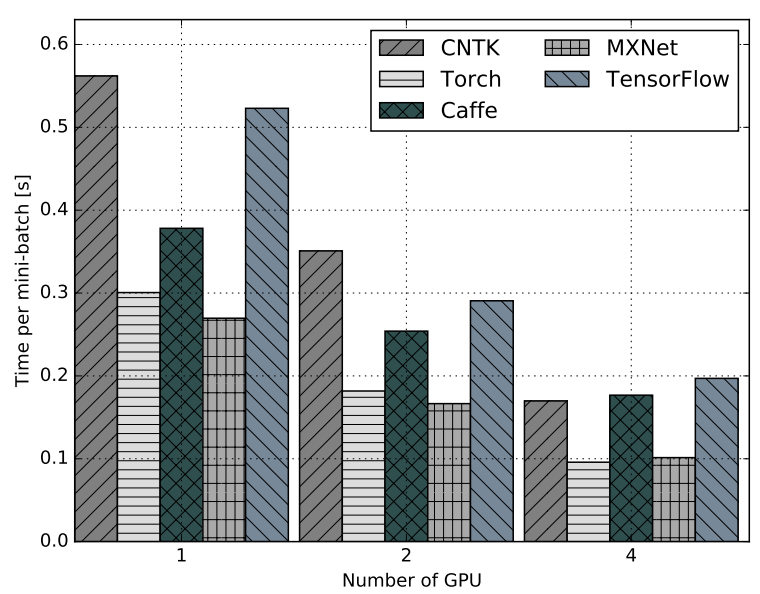
\includegraphics[width=0.4\textwidth]{a.png}

\caption{Time per mini-batch in s compared between different amount of GPUs used\cite{shi2016benchmarking}}
\label{fig_m_gpu}
\end{figure}

\subsection{GPU-Clusters}

The next logical step is to use multiple Multi-GPU systems further reducing training time but also creating new challenges, because of the decentralized nature of the Cluster, like communication overhead.  This is mostly used in large scale applications and is most of the time not needed in small scale.

\begin{figure}
\centering
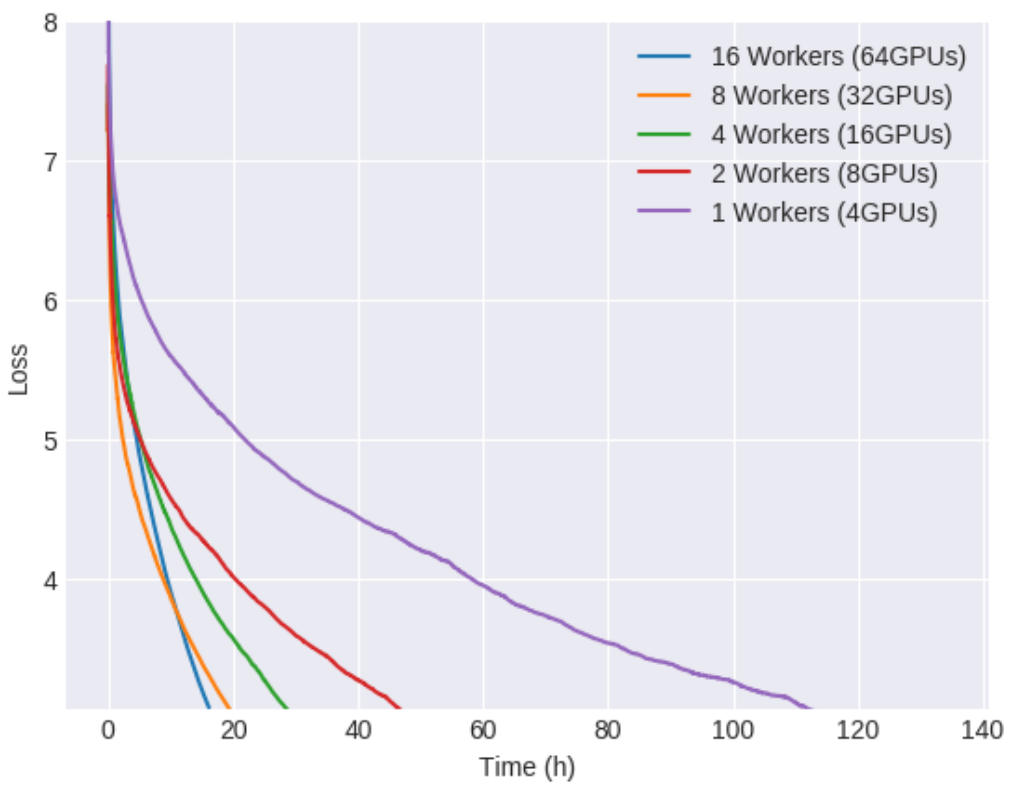
\includegraphics[width=0.4\textwidth]{gpu_cluster_perf_win.png}
\caption{Time (in h) of different asynchronous configurations until reaching destined error rate(loss)\cite{sastre2017scalability}}
\label{fig_cl_gpus}
\end{figure}

\subsubsection{Multiple GPU-Clusters}
Taking a step further it is possible to connect multiple Clusters of GPUs to compute a single task. In doing this we again increase raw computation power, but also increase the total amount of communication required. Similar to multiple GPUs this leads at the beginning with 2 or more Clusters to a stronger improvement than later on with 8 to 16 Clusters as seen in (Fig. 2)

\subsubsection{Parallelism of multiple GPU-Clusters}
Like the Multi-GPU setup this can be done by creating either data or model parallelism. Combination are also possible when using GPU-Clusters, for instance in a setup consisting of multiple Clusters and one single communication server a model parallelism can be used to distribute the model on the different clusters, but they internally use data parallelism to split work\cite{wang2016deep}.

\subsubsection{Synchronization of multiple GPU-Clusters}
Similar to parallelism the synchronization of GPU-Clusters can be undertaken either with the synchronous or asynchronous like in Multi-GPU configurations. Again these tactics can be combined to create a mixed-asynchronous strategy, using an asynchronus training on inter-clusters level and cluster internal synchronous training\cite{sastre2017scalability}. This creates the best performance on large configurations with many clusters\cite{wang2016deep}.

%%%%%%%%%%%%%%%%%%%%%%%%%%%%%%%%%%%%%%%%%%%%%%%%%BEGIN CHALLENGES


\section{Large scale challenges and Small scale challenges}
Dependent on the choice of scale each one has its own challenges to be considered during design and implementation of the neural network.

\subsection{Small scale challenges}
First and foremost it is important to notice that the biggest restrictions of small scale applications is the limited computation power available during the initial training process, later during usage of the net this is less impeding because either the net is completely pretrained and not changed later or the only change is some optimization when the network receives a query.

This leads to the focus lying on the design to find the best fit of complexity to fit the desired model. Otherwise longer training time or less accuracy of the resulting network will conclude.

Further small scale applications are relatively free of performance related complications, because of their relative simplicity and fast modern computer hardware enabling operations which are not optimal to be resolved in a non less desirable time.

\subsection{Large scale challenges}
Opposing to small scale applications large scale ones to not have the actual processing power as their highest pending restriction but the communication and data transfer between all acting processing units. This problem occurs because a larger data flow has to be managed to more processing units compared to small scale applications.

\begin{figure}
\centering
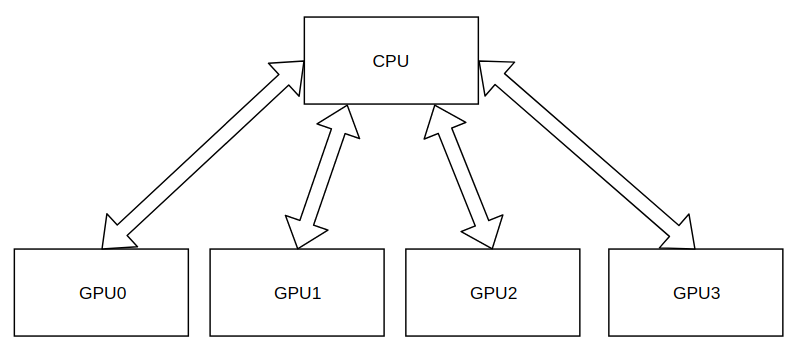
\includegraphics[width=0.4\textwidth]{example_configuration.png}
\caption{One example configuration consisting of a CPU and 4 connected GPU units for training the neural network.}
\end{figure}

%%Data flow of training data
The data flow is a problem on multiple fronts. For one the transfer of the training data from main memory to GPU memory can be the first bottleneck restricting faster processing speeds from being realized. For example if the GPU only receives data if no calculation is currently active this slows down the training process unnecessarily. To increase the speed of the calculation data can be fetched during the processing of already present data, this is called data prefetching as described and implemented by Yang 2010 \cite{yang2010gpgpu}. This solution can solve the problem partially but reaches it limits if used with multiple GPUs for example configuration (Fig. 3), which leads that the CPU will become a bottleneck if the training data of each individual GPU is too large to fit in the GPU memory, since the CPU can only manage transfer to the GPUs one at a time. For example a GPU equipped with PCI-Express 4.0 with a x16 Throughput can at best receive 31.5 GB/s, if we assume that all training data can be fit into main memory, that way if we need to refresh the complete memory of a modern GPU like NVIDIA GTX 1080, we need 0.253968 s, so to refresh all GPUs memory without including any overhead produced by switching operations between the GPUs we have an absolute transfer time of 1.015873 s, and for 3 units 0.7619 s, so if our GPU completes the desired calculation faster, for example 0.5 s, we have an 0.2619 s period in which our GPU idles every iteration, assumed that we can transfer all data during the calculation time. Therefore we have an effective calculation computation time each phase of 65.62 \%. This problem only enlargens if the main memory is to small to fit the complete training data since connections to solid state disk are too slow and hard disk do physically do not reach the required throughput.

%%data flow synchronization
Additional data flow is created when synchronizing GPUs with each other, by approaches described beforehand in "Choice of Processing Units", they each have their own advantage but can limit efficiency in certain situations. But both create an communication overhead because during transmission of values the GPU cannot operate on the neural network training.

\begin{figure}
\centering
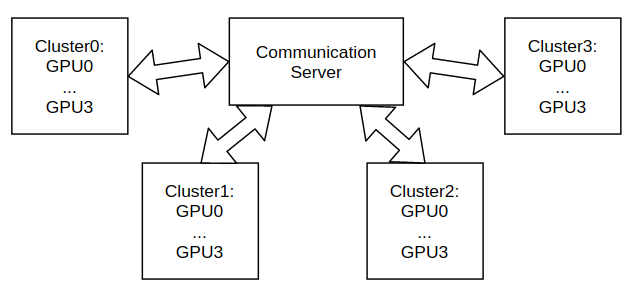
\includegraphics[width=0.4\textwidth]{cluster_setup.png}
\caption{One example configuration consisting of a communication server and 4 connected GPU-Clusters each containing 4 GPUs.}
\end{figure}
%synchronous
Synchronous training, while being recommend for setups that have 40 GPUs or less, can create idling time if one unit is slower than others, since all updates have to be send to the server before the next iteration can be undertaken this slows down all other units. This problem becomes more probable the more units are used. Also more GPUs lead to more communication if synchronization is required after very step, so they increase the amount of data managed by the CPU or communication server. This applies to configuration like Figure 3 and Figure 4.

%asynchronous
If an asynchronous training approach is used problems may occur influencing the result, if updates are to sporadic and different versions of values drift too far apart. To avoid this problem GPU-Cluster configurations do not rely on complete asynchronous training startegies, but on the already described mixed-asynchronous minimizing this problem while still reducing possible communication overhead.

To ease the effect of GPU to GPU communication,by relieveing the CPU of managing them, technologies like GPUDirect from NVIDIA\cite{nvidiagpudirect2017} can be used allowing direct GPU to GPU communication if they are connected to the same PCIe bus, so this is only appplicable within a GPU Cluster or a single system and does not remove all communication overhead. Also shared memory between GPUs can come in place saving synchronization between them.

%memory limitation
Another issue appears while training if the training data is too large to fit in memory. Then time expensive disk accesses to either very slow HDDs or faster but still relatively slow SSDs are required. For example a fast available SSD SAMSUNG 960 PRO can reach up to 3.5 GB/s which is still relatively slow compared to the maximum 31.5 GB/s possible through an PCIe x16 interface. To further increase speed a RAID 0 setup can be created consisting of multiple M.2 SSDs with the potential of parallel access and data transfer reaching for instance with 5 960 PRO that could transfer at maximum of around 17 GB/s.

%bandwith between clusters
This data transfer becomes only more and more concerning if multiple GPU-Cluster are used, because the connection between them may slower than the interfaces of RAM, GPU and storage used therefore creating a new bottleneck. This problem can be reduce if training data is stored by the cluster, which has the downside of further increasing the cost of these setups.


%%%%%%%%%%%%%%%%%%%%%%%%%%%%%%%%%%%%%%%%%%%%%%%%%BEGIN CONCLUSION


\section{Conclusion}
%Summary
During our survey we observed that the most influencing factors are the basic choice of neural network to be used, this includes its complexity as well as the actual architecture the network is build of. Further the processing unit that is chosen has a strong influence on the quality and speed the final network that lies within acceptable error limits will be reached. Based on the choice of this other factors came into consideration influencing the process, like communication between processing units and parallelism of data between them. They are not quite as influential as the first two but can lead to a strong improvement or worsening. We observed that even in example systems that handle communication efficiently about 35 \% of the calculation time is sacrificed to it.

%Takeaway
Especially data transfer time and alike carries a potential to lengthen the training time of an significant amount. To ease this technology like GPUDirect\cite{nvidiagpudirect2017} and data prefetching\cite{yang2010gpgpu} can be used. It may be possible to decrease the effect of the data flow further by introducing a direct memory transfer unit which can indepently organize synchronization and can handle parallel transfers to and from multiple GPUs. This could decrease the calculation time to a bare minimum but would require additional hardware and maybe modification of the used GPUs. Although this could break some security limits because of unauthorized memory accesses. 

% use section* for acknowledgment
\section*{Acknowledgment}
The author would like to thank Gabriel Campero Durand for advise and help to write the paper


% trigger a \newpage just before the given reference
% number - used to balance the columns on the last page
% adjust value as needed - may need to be readjusted if
% the document is modified later
%\IEEEtriggeratref{8}
% The "triggered" command can be changed if desired:
%\IEEEtriggercmd{\enlargethispage{-5in}}

\bibliographystyle{IEEEtran}
\bibliography{paper}


% that's all folks
\end{document}


